\begin{figure*}
	\centering
    \resizebox{1.5\columnwidth}{!}{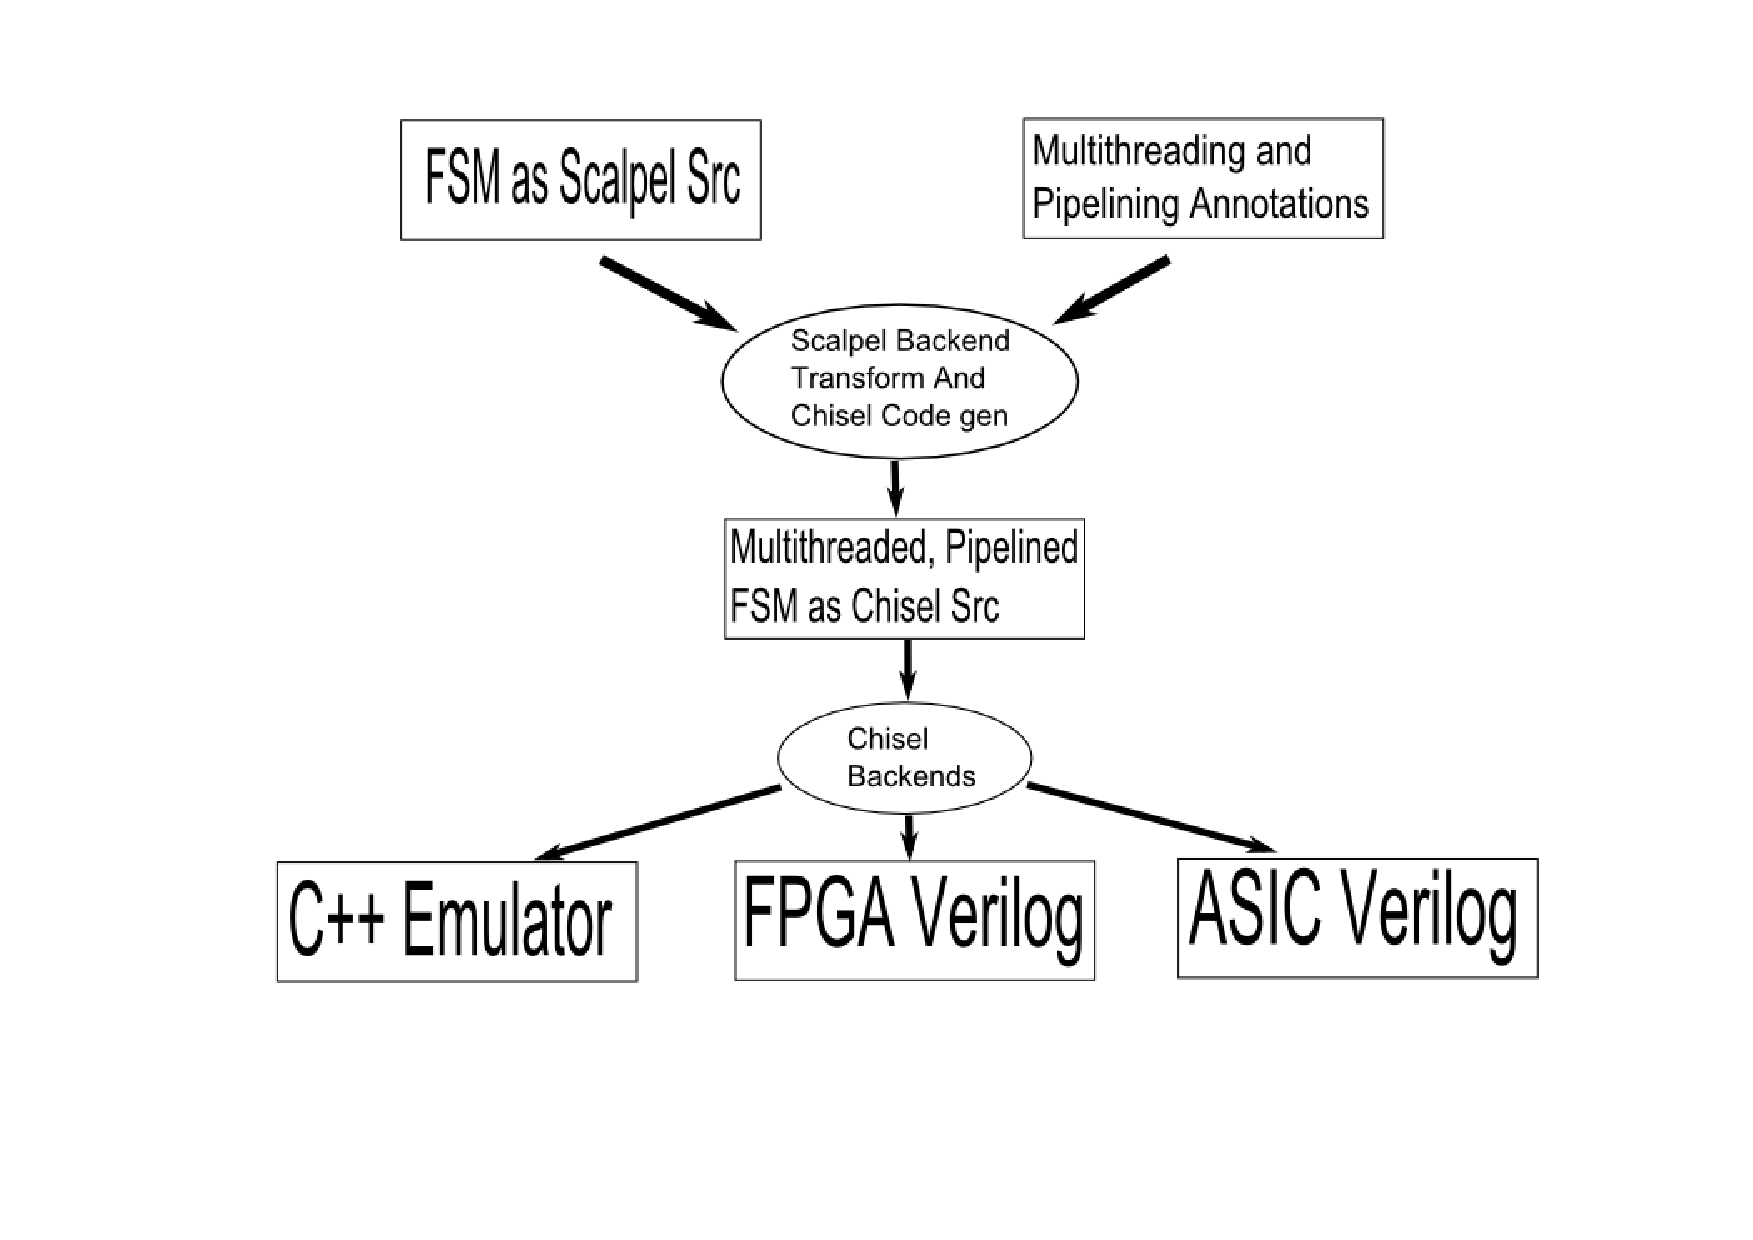
\includegraphics{figures/workflow}}
    \caption{Overall Tool Flow}
	\label{fig:workflow}
\end{figure*}

\section{Proposed Solution}
HLS produces designs with unacceptable performance/power/area tradeoffs because the synthesis tool has to solve the computationally difficult problem of formulating a datapath that executes the dataflow graph and fits within the given performance/power/area constraints. HLS tools do synthesize well optimized designs for specific patterns that occur in the high-level specification, so hardware designers working with HLS find themselves tuning high-level code to make specific synthesis tools produce exactly the datapath they want. 

This is clearly a case of automation trying to do too much. The HLS tools have a hard time formulating optimized datapaths, so the designers have to essentially tell the HLS tools what datapath they should use in a roundabout way by tuning the high-level specification. Clearly, designers would be more productive if they can specify the datapath directly. 

It seems like this conclusion tells us that designers should just do logic design using RTL in the traditional manner. However, much of traditional RTL specification deals with issues outside of simple datapath design. Logic designers spend much of their time specifying additional logic required to make the datapath fit performance/power/area constraints. Some common optimization techniques include time-multiplexing functional units, pipelining, multi-threading, out-of-order execution, etc. These commonly used datapath optimization techniques can be captured as algorithms and applied automatically.

This paper proposes a system in which the designer specifies in RTL a minimally complex finite state machine (FSM) that is functionally correct , but has no optimizations applied to it. The designer then annotates the minimal circuit with desired optimizations in the RTL source file and uses a software tool to automatically apply the optimizations to the minimal FSM. It is useful to have the annotations that specifiy optimizations to be used be placed directly in the RTL src file because it allows the user to refer to variables present in the RTL when specifying ooptimizations. The tool described in this paper is capable of creating multi-thread in-order designs of any number of threads and any number of pipeline stages that is functionally equivalent to n-copies of the original minimal FSM, where n is the number of threads. 

The tool supports two types of multi-threading, fixed and dynamic interleave. In fixed interleave, the tool uses a fixed counter to select the next thread to wake up. The tool enforces that the number of threads is greater than or equal to the number of pipeline stages, so there can not be any data hazards between any two transactions in the pipeline because there is always at most one transaction from each thread in the pipeline. This allows the tool to not generate the data dependency check and resolution logic. Additionally, in fixed interleave, the tool does not generate logic to retry a transaction if it encounters a Resp Pending from a Variable Latency Unit Interface. Instead, the whole pipeline stalls. In dynamic pipelining, the tool uses a user supplied thread scheduler that selects the next thread to wake up based on the status of any long latency functional units in that thread. In this mode, even if the tool restricts the number of threads to be greater than or equal to the number of pipeline stages, data hazards between two transactions in the pipeline cannot be avoided because the user supplied scheduler is free to choose any thread order and there for can place more than one transaction from each thread in the pipeline. Additionally, in dynamic interleave, the tool generate logic to retry a transaction if it encounters a Resp Pending from a Variable Latency Unit Interface and does not stall the pipeline.

The RTL specification language used in this paper is a reduced version of Chisel\cite{Bachrach:2012}, a HDL developed by UC Berkeley. Chisel is particularly suited for this project because unlike Verilog and VHDL, it specifies digital circuits through explicit circuit component construction, not inference based on a discrete event simulator semantics. This means that Chisel internally holds a representation of the digital circuit specified by the designer as an easily manipulatable node graph. The tool takes advantage of this fact and creates the multi-threaded, pipelined designs by adding to and modifying the Chisel internal node graph of the original FSM. A reduced version of Chisel is used for this paper to help constrain the scope of the project and to produce initial results. This reduced version of Chisel will be refered to as Scalpel for the rest of this paper. In the future, the system will be extended to work with Chisel.

The automatic optimization tool described in this paper extends a previous class project that implemented a system that automatically generates in order pipelined designs from a minimal FSM specified in Chisel. There are many shared features and components between this tool and the old tool. This paper will focus on the automatic multi-threading parts of the tool.

Figure \ref{fig:workflow}. shows the flow of the entire system. The designer first creates in Scalpel a ISA simulator like minimal FSM that does not have any optimizations implemented. The also designer annotates the Scalep source file with the number threads, dynamic or fixed interleave, and the number of pipeline stages. Then the automatic transformation tool, which is implemented as a transformation that manipulates Scalpel's internal node graph representation of the original minimal FSM. The Scalpel code generator then takes the modified node graph and generates a Chisel source file that represents the multi-threaded, pipelined version of the original minimal FSM that is functionally identical to n copies of the minimal FSM, where n is the number of threads. Then the Chisel elaborator will use the generated Chisel source file to generate a cycle accurate C++ emulator or Verilog source file.
